\documentclass[]{article}
\usepackage{lmodern}
\usepackage{amssymb,amsmath}
\usepackage{ifxetex,ifluatex}
\usepackage{fixltx2e} % provides \textsubscript
\ifnum 0\ifxetex 1\fi\ifluatex 1\fi=0 % if pdftex
  \usepackage[T1]{fontenc}
  \usepackage[utf8]{inputenc}
\else % if luatex or xelatex
  \ifxetex
    \usepackage{mathspec}
  \else
    \usepackage{fontspec}
  \fi
  \defaultfontfeatures{Ligatures=TeX,Scale=MatchLowercase}
\fi
% use upquote if available, for straight quotes in verbatim environments
\IfFileExists{upquote.sty}{\usepackage{upquote}}{}
% use microtype if available
\IfFileExists{microtype.sty}{%
\usepackage{microtype}
\UseMicrotypeSet[protrusion]{basicmath} % disable protrusion for tt fonts
}{}
\usepackage[margin=1in]{geometry}
\usepackage{hyperref}
\hypersetup{unicode=true,
            pdftitle={MT4113: Assignment 3, Monte Carlo Simulation},
            pdfauthor={180024570},
            pdfborder={0 0 0},
            breaklinks=true}
\urlstyle{same}  % don't use monospace font for urls
\usepackage{graphicx,grffile}
\makeatletter
\def\maxwidth{\ifdim\Gin@nat@width>\linewidth\linewidth\else\Gin@nat@width\fi}
\def\maxheight{\ifdim\Gin@nat@height>\textheight\textheight\else\Gin@nat@height\fi}
\makeatother
% Scale images if necessary, so that they will not overflow the page
% margins by default, and it is still possible to overwrite the defaults
% using explicit options in \includegraphics[width, height, ...]{}
\setkeys{Gin}{width=\maxwidth,height=\maxheight,keepaspectratio}
\IfFileExists{parskip.sty}{%
\usepackage{parskip}
}{% else
\setlength{\parindent}{0pt}
\setlength{\parskip}{6pt plus 2pt minus 1pt}
}
\setlength{\emergencystretch}{3em}  % prevent overfull lines
\providecommand{\tightlist}{%
  \setlength{\itemsep}{0pt}\setlength{\parskip}{0pt}}
\setcounter{secnumdepth}{5}
% Redefines (sub)paragraphs to behave more like sections
\ifx\paragraph\undefined\else
\let\oldparagraph\paragraph
\renewcommand{\paragraph}[1]{\oldparagraph{#1}\mbox{}}
\fi
\ifx\subparagraph\undefined\else
\let\oldsubparagraph\subparagraph
\renewcommand{\subparagraph}[1]{\oldsubparagraph{#1}\mbox{}}
\fi

%%% Use protect on footnotes to avoid problems with footnotes in titles
\let\rmarkdownfootnote\footnote%
\def\footnote{\protect\rmarkdownfootnote}

%%% Change title format to be more compact
\usepackage{titling}

% Create subtitle command for use in maketitle
\newcommand{\subtitle}[1]{
  \posttitle{
    \begin{center}\large#1\end{center}
    }
}

\setlength{\droptitle}{-2em}

  \title{MT4113: Assignment 3, Monte Carlo Simulation}
    \pretitle{\vspace{\droptitle}\centering\huge}
  \posttitle{\par}
    \author{180024570}
    \preauthor{\centering\large\emph}
  \postauthor{\par}
      \predate{\centering\large\emph}
  \postdate{\par}
    \date{21/11/2018}

\usepackage{subfig}
\usepackage{booktabs}
\usepackage{longtable}
\usepackage{array}
\usepackage{multirow}
\usepackage[table]{xcolor}
\usepackage{wrapfig}
\usepackage{float}
\usepackage{colortbl}
\usepackage{pdflscape}
\usepackage{tabu}
\usepackage{threeparttable}
\usepackage{threeparttablex}
\usepackage[normalem]{ulem}
\usepackage{makecell}

\usepackage{booktabs} \usepackage{longtable} \usepackage{array} \usepackage{enumitem} \usepackage{multirow} \usepackage[table]{xcolor} \usepackage{wrapfig} \usepackage{float} \floatplacement{figure}{H} \usepackage[bottom]{footmisc}

\begin{document}
\maketitle

\emph{I confirm that the following report and associated code is my own
work, except where clearly indicated.}

\hypertarget{abstract}{%
\section{Abstract}\label{abstract}}

More than 17 million people voted to leave the EU in 2016 Referendum in
the UK. This statistical report investigated the difference of approval
rates of Brexit in England and the rest of the UK by carrying out both
parametric and non-parametric tests. Particularly, Monte Carlo
simulation is conducted on the referendum dataset by regions, to
research the properties of those statistical tests under a range of
different scenarios.

\hypertarget{motivation}{%
\section{Motivation}\label{motivation}}

Hundreds of thousands of people marched to London's Parliament Square
for a referendum on the final Brexit deal in late October(BBC News,
2018). In the EU referendum in 2016, approximately 52\%, or more than 17
million people in the UK, voted to leave the European Union (Becker,
Fetzer \& Novy, 2017). To investigate what voters in different nations
of the UK vote for, the dataset of EU referendum results by
regions(Electoral Commission, 2016) are statistically analysed and
tested in this report. The dateset contains numerous variates regarding
the referendum outcome, yet only \emph{Region} and \emph{Percent Leave}
are concerned in terms of our research objectives.

\begin{figure}
\centering
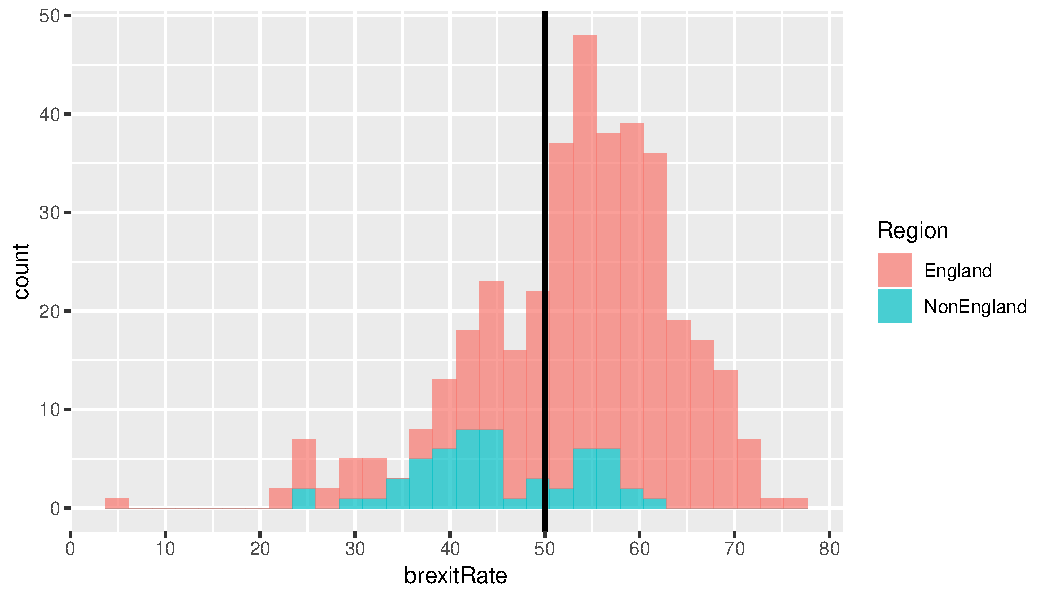
\includegraphics{../figure/datasetHist.pdf}
\caption{Vote Outcome in England and Non-England Regions}
\end{figure}

According to the histogram of leave votes, it seems that England regions
tend to be more supportive of Brexit than other regions. Hence, The
research question is proposed as that

\begin{itemize}
\tightlist
\item
  \emph{Were approval rates of Brexit Higher in England than rest of the
  UK in 2016 referendum?}
\end{itemize}

On the basis of our research question, regions are categorized as
England or Non-England, thus, One-tail Student's T test and Mann-Whitney
U test are chosen to be conducted to compare the difference of mean
approval rates of Brexit. Moreover, 1000-iteration Monte Carlo
simulations are carried out under a range of scenarios in order to
investigate power and size of these tests.

\hypertarget{methodology}{%
\section{Methodology}\label{methodology}}

\hypertarget{data-exploration-and-tests-specification}{%
\subsection{Data Exploration and Tests
Specification}\label{data-exploration-and-tests-specification}}

By organizing and exploring dataset \emph{Referendum}, the properties of
leave vote rates are summarized in table 1. It shows that the Brexit
approval rate in England regions was approximate 10\% higher than in
Non-England regions on average. In general, England tended to leave the
EU with leave vote rate more than a half, while other nations tended to
remain with leave vote rate less than 50\%.

\begin{longtable}[t]{lrrr}
\caption{\label{tab:dataset}Summary of Leave Vote Rates in Regions of England and Non-England}\\
\toprule
Region & n & mean & sd\\
\midrule
England & 327 & 54.35 & 10.38\\
NonEngland & 55 & 44.91 & 8.88\\
\bottomrule
\end{longtable}

What is concerned in this research is whether the leave vote rates in
England regions \emph{higher} than in Non-England regions, which
involves two groups of samples. Therefore, the statistical tests to be
conducted should be one-tailed test for two groups. The chosen tests are

\begin{itemize}
\item
  Parametric: One-tailed Student's t Test
\item
  Non-parametric: One-tailed Mann-Whitney U Test
\end{itemize}

The null Hypothesis and alternative hypothesis are

\begin{itemize}
\item
  \(H_0\): \(\mu_{e} - \mu_{o} \le 0\)
\item
  \(H_1\): \(\mu_{e} - \mu_{o} > 0\)
\end{itemize}

where \(\mu_{e}\) is the mean leave vote rate in England, and
\(\mu_{o}\) is the mean leave vote rate in the rest of the UK.

\hypertarget{scenario-design}{%
\subsection{Scenario Design}\label{scenario-design}}

Scenario design and data simulation are grounded on the properties shown
in table 1 in previous section.

To investigate the \emph{power} of two tests, the difference of mean
leave vote rates, a.k.a. the effect size, are set to be positive, where
\(H_0\) is false. The specific effect sizes of simulating data are
chosen to be 1\%, 3\%, 6\%, 10\%, and 15\%, covering scenarios under
which the mean differences are less than, close to, or greater than the
actual mean difference 9.4\%. The steps between those effect sizes are
incremental, because it is speculated that the power of a test is more
responsive in smaller scale. The standard deviation are set to be 10\%
for England group and 8\% for Non-England group, which is close to the
true properties.

To investigate the \emph{size} of two tests, the effect sizes are set to
be 0, where \(H_0\) is true. There are two groups of scenarios, one
simulated with all percentage records rounded to 0, another as default.
For each scenario of one group, the difference of standard deviation are
set to be 0\%, 3\%, 5\%, 10\%.

For each attributes stated above, 10 datasets of different sample sizes
from 10 to 1000 are generated to be test.

\hypertarget{monte-carlo-simulation}{%
\subsection{Monte Carlo Simulation}\label{monte-carlo-simulation}}

Two functions are created to complete the workflow. Function
\texttt{simulating()} generates a dataset given conditions of scenario,
e.g.~sample size, mean and standard deviation of two groups of datasets.
Function \texttt{MonteCarlo()} invokes \texttt{simulating()}, carries
out specific test and stores the \(p\)-value, by doing all these 1000
iterations it finally return the proportion of rejecting \(H_0\). The
number of iteration, parametric or non-parametric test to be conducted
are also arbitrary and can be specified as inputs. Also, both functions
have a \emph{seed} argument for reproducibility purpose.

A 10 by 5 \emph{power} matrix is evaluated for t test and Mann-Whitney U
test respectively. 10 rows are for 10 different sample sizes, 5 columns
are for different effect sizes. Similarly, two 10 by 8 \emph{size}
matrices are evaluated for two tests, 8 columns are for 4 differences of
standard deviation and round to 0 or not.

\hypertarget{result-and-discussion}{%
\section{Result and Discussion}\label{result-and-discussion}}

Each cell of the \emph{power} matrix is calculated based on 1000 times
of test, and the outcomes for are t test and Mann-Whitney U test are
respectively shown in table 2 and table 3.

\begin{table}[!htb]
    \begin{minipage}{.5\linewidth}
      \centering 
\begin{longtable}[t]{lrrrrr}
\caption{\label{tab:power-tables}Power of Student's T Test}\\
\toprule
\multicolumn{1}{c}{\bfseries Sample Size} & \multicolumn{5}{c}{\bfseries Effect Size (Unit: \%)} \\
\cmidrule(l{2pt}r{2pt}){1-1} \cmidrule(l{2pt}r{2pt}){2-6}
  & 1 & 3 & 6 & 10 & 15\\
\midrule
10 & 0.000 & 0.009 & 0.32 & 0.953 & 1\\
50 & 0.000 & 0.510 & 1.00 & 1.000 & 1\\
100 & 0.000 & 1.000 & 1.00 & 1.000 & 1\\
150 & 0.000 & 1.000 & 1.00 & 1.000 & 1\\
200 & 0.001 & 1.000 & 1.00 & 1.000 & 1\\
\addlinespace
300 & 0.047 & 1.000 & 1.00 & 1.000 & 1\\
400 & 0.296 & 1.000 & 1.00 & 1.000 & 1\\
500 & 0.720 & 1.000 & 1.00 & 1.000 & 1\\
700 & 0.995 & 1.000 & 1.00 & 1.000 & 1\\
1000 & 1.000 & 1.000 & 1.00 & 1.000 & 1\\
\bottomrule
\end{longtable} \end{minipage}%
    \begin{minipage}{.5\linewidth}
      \centering 
\begin{longtable}[t]{lrrrrr}
\caption{\label{tab:power-tables}Power of Mann-Whitney U Test}\\
\toprule
\multicolumn{1}{c}{\bfseries Sample Size} & \multicolumn{5}{c}{\bfseries Effect Size (Unit: \%)} \\
\cmidrule(l{2pt}r{2pt}){1-1} \cmidrule(l{2pt}r{2pt}){2-6}
  & 1 & 3 & 6 & 10 & 15\\
\midrule
10 & 0.001 & 0.016 & 0.358 & 0.92 & 1\\
50 & 0.000 & 0.565 & 1.000 & 1.00 & 1\\
100 & 0.000 & 0.998 & 1.000 & 1.00 & 1\\
150 & 0.003 & 1.000 & 1.000 & 1.00 & 1\\
200 & 0.009 & 1.000 & 1.000 & 1.00 & 1\\
\addlinespace
300 & 0.072 & 1.000 & 1.000 & 1.00 & 1\\
400 & 0.305 & 1.000 & 1.000 & 1.00 & 1\\
500 & 0.634 & 1.000 & 1.000 & 1.00 & 1\\
700 & 0.975 & 1.000 & 1.000 & 1.00 & 1\\
1000 & 1.000 & 1.000 & 1.000 & 1.00 & 1\\
\bottomrule
\end{longtable} \end{minipage} 
\end{table}

The result suggests that, for both parametric and non-parametric tests,
small effect size like 1 results in low power, even 0 power. With sample
size increasing, the power of test also increases. Under scenarios with
small sample size, the power of test is positively related to the effect
size. Even sample size is as small as 10, the power can be appreciably
high when effect size reach 10 or greater.

By plotting the power over sample size(fig. 2), it is clear to see that
sample size is also positively related to power of tests. Besides, the
plots indicate that there is no sensible power difference between
parametric and non-parametric tests under same scenario. The sample
sizes of two groups in the true dataset are respectively 327 and 55, and
the mean difference of two samples are round 10. In this case, both t
test and Mann-Whitney test have significant power estimates.

\begin{figure}
\centering
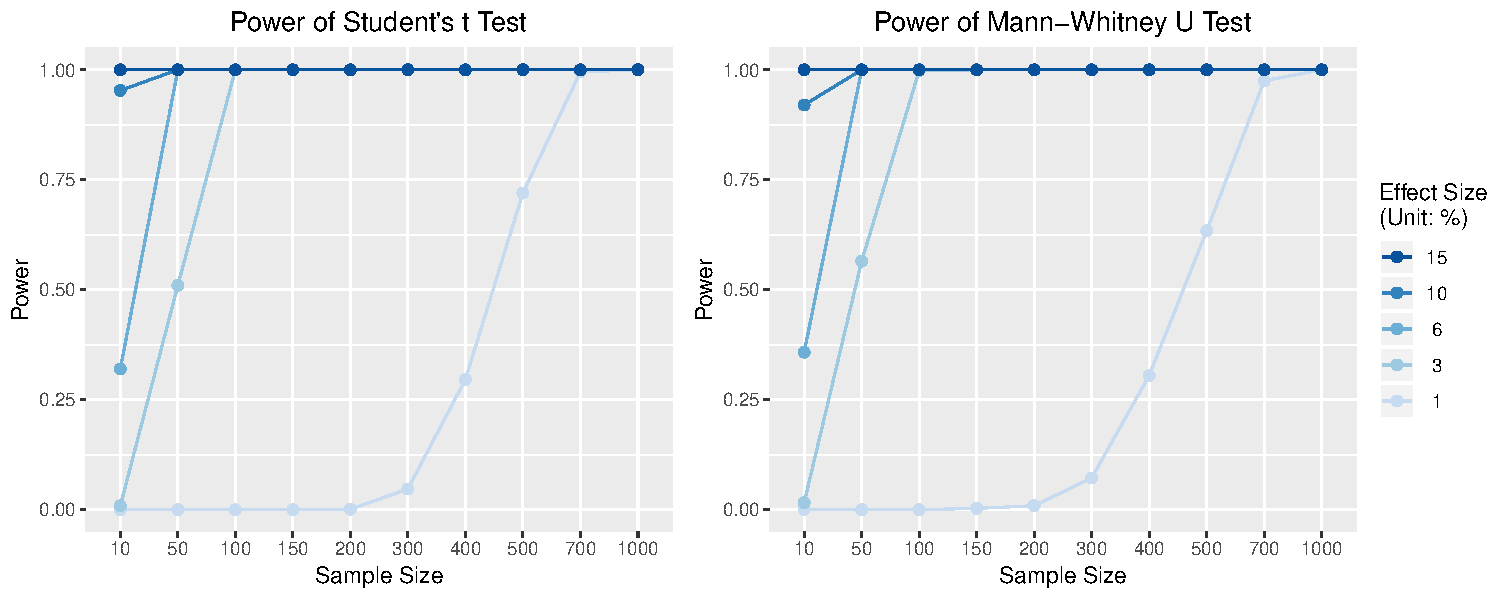
\includegraphics{../figure/power.pdf}
\caption{Power of Parametric and Non-parametric Tests under Different
Scenarios}
\end{figure}

Likewise, each cell of the \emph{size} matrix is calculated based on
1000 times of test, and the outcomes for are t test and Mann-Whitney U
test are respectively shown in table 4 and 5. The \emph{size} matrix
suggest that, the larger the difference of standard deviation is, the
higher the sizes of tests are, given identical sample size. When the
difference is 0, the size is always zero.

\begin{longtable}[t]{lrrrrrrrr}
\caption{\label{tab:size-tables}Size of Student's T Test}\\
\toprule
\multicolumn{1}{c}{\bfseries Sample Size} & \multicolumn{4}{c}{\bfseries SD Difference} & \multicolumn{4}{c}{\bfseries SD Difference(rounded)} \\
\cmidrule(l{2pt}r{2pt}){1-1} \cmidrule(l{2pt}r{2pt}){2-5} \cmidrule(l{2pt}r{2pt}){6-9}
  & 0 & 3 & 5 & 10 & 0 & 3 & 5 & 10\\
\midrule
10 & 0 & 0.017 & 0.025 & 0.032 & 0 & 0.014 & 0.025 & 0.035\\
50 & 0 & 0.009 & 0.022 & 0.034 & 0 & 0.011 & 0.017 & 0.035\\
100 & 0 & 0.012 & 0.020 & 0.023 & 0 & 0.014 & 0.020 & 0.024\\
150 & 0 & 0.019 & 0.027 & 0.031 & 0 & 0.019 & 0.026 & 0.030\\
200 & 0 & 0.009 & 0.021 & 0.025 & 0 & 0.010 & 0.017 & 0.028\\
\addlinespace
300 & 0 & 0.010 & 0.022 & 0.034 & 0 & 0.011 & 0.025 & 0.036\\
400 & 0 & 0.019 & 0.029 & 0.038 & 0 & 0.018 & 0.030 & 0.041\\
500 & 0 & 0.016 & 0.025 & 0.039 & 0 & 0.015 & 0.025 & 0.038\\
700 & 0 & 0.013 & 0.022 & 0.034 & 0 & 0.013 & 0.020 & 0.033\\
1000 & 0 & 0.015 & 0.029 & 0.036 & 0 & 0.013 & 0.028 & 0.036\\
\bottomrule
\end{longtable}

\begin{longtable}[t]{lrrrrrrrr}
\caption{\label{tab:size-tables}Size of Mann-Whitney U Test}\\
\toprule
\multicolumn{1}{c}{\bfseries Sample Size} & \multicolumn{4}{c}{\bfseries SD Difference} & \multicolumn{4}{c}{\bfseries SD Difference(rounded)} \\
\cmidrule(l{2pt}r{2pt}){1-1} \cmidrule(l{2pt}r{2pt}){2-5} \cmidrule(l{2pt}r{2pt}){6-9}
  & 0 & 3 & 5 & 10 & 0 & 3 & 5 & 10\\
\midrule
\endfirsthead
\caption[]{Size of Mann-Whitney U Test \textit{(continued)}}\\
\toprule
\multicolumn{1}{c}{\bfseries Sample Size} & \multicolumn{4}{c}{\bfseries SD Difference} & \multicolumn{4}{c}{\bfseries SD Difference(rounded)} \\
\cmidrule(l{2pt}r{2pt}){1-1} \cmidrule(l{2pt}r{2pt}){2-5} \cmidrule(l{2pt}r{2pt}){6-9}
  & 0 & 3 & 5 & 10 & 0 & 3 & 5 & 10\\
\midrule
\endhead
\
\endfoot
\bottomrule
\endlastfoot
10 & 0 & 0.029 & 0.041 & 0.049 & 0 & 0.031 & 0.047 & 0.057\\
50 & 0 & 0.028 & 0.046 & 0.057 & 0 & 0.031 & 0.047 & 0.058\\
100 & 0 & 0.028 & 0.048 & 0.065 & 0 & 0.029 & 0.045 & 0.070\\
150 & 0 & 0.033 & 0.049 & 0.057 & 0 & 0.032 & 0.045 & 0.057\\
200 & 0 & 0.026 & 0.045 & 0.061 & 0 & 0.028 & 0.047 & 0.061\\
\addlinespace
300 & 0 & 0.036 & 0.051 & 0.071 & 0 & 0.034 & 0.056 & 0.075\\
400 & 0 & 0.043 & 0.064 & 0.080 & 0 & 0.044 & 0.064 & 0.080\\
500 & 0 & 0.034 & 0.051 & 0.066 & 0 & 0.027 & 0.051 & 0.069\\
700 & 0 & 0.029 & 0.048 & 0.057 & 0 & 0.034 & 0.050 & 0.062\\
1000 & 0 & 0.038 & 0.054 & 0.071 & 0 & 0.037 & 0.056 & 0.070\\*
\end{longtable}

By visualizing the two verbose tables(see fig. 3), it is obvious that,
in contrast to power, the size of test does not vary over sample size.
The true difference of sample standard deviations is 1.5\%, falling
between 0\% and 3\%, resulting relatively low size for both tests. Also,
there is no distinct effect of rounding percentage of vote rate to
integer. However, the different scale of y-asix is one thing worth
noticing, which indicates that the size of Mann-Whitney test is greater
than t test in general.

\begin{figure}
\centering
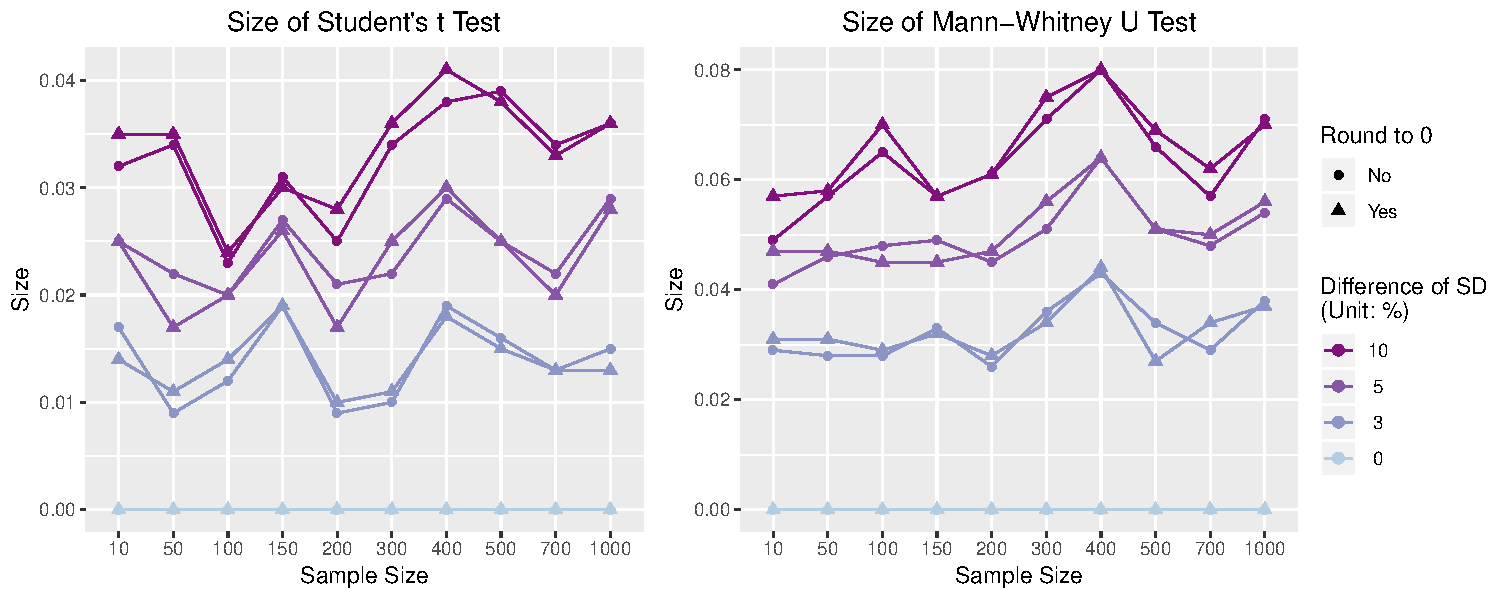
\includegraphics{../figure/size.pdf}
\caption{Size of Parametric and Non-parametric Tests Under Different
Scenarios}
\end{figure}

In summary, effect size and variance have considerable impacts on power
and size of tests, but there is not much can be done to the properties
of population. Nevertheless, the result analysis does indicate that
larger sample size leads to greater power of test, and parametric test
shows better performance with smaller size under identical scenario.

\hypertarget{conclusion}{%
\section{Conclusion}\label{conclusion}}

Both t test and Mann-Whitney U test rejected the null hypothesis, and
these tests has convincible power and size according to the result
analysis of Monte Carlo simulation. We can statistically infer that the
approval rates of Brexit were higher in England than rest of the UK in
2016 referendum.

Generally, we can also conclude that it is prudent to enlarge the sample
size to reach higher power of test and choose parametric test when we
can assume the distribution of population.

\newpage

\hypertarget{reference}{%
\section{Reference}\label{reference}}

\hypertarget{refs}{}
\leavevmode\hypertarget{ref-BBCNews2018}{}%
BBC News (2018) \emph{People's Vote march: Hundreds of thousands attend
London protest}. {[}Online{]}. Available from:
\url{https://www.bbc.co.uk/news/uk-45925542}.

\leavevmode\hypertarget{ref-Becker2017}{}%
Becker, S.O., Fetzer, T. \& Novy, D. (2017) Who voted for Brexit? A
comprehensive district-level analysis. \emph{Economic Policy}.
{[}Online{]} Available from:
doi:\href{https://doi.org/10.1093/epolic/eix012}{10.1093/epolic/eix012}.

\leavevmode\hypertarget{ref-ElectoralCommission2016}{}%
Electoral Commission (2016) \emph{2016 EU Referendum in the United
Kingdom}. {[}Online{]}. Available from:
\url{https://www.kaggle.com/electoralcommission/brexit-results}.

\leavevmode\hypertarget{ref-ggpubr}{}%
Kassambara, A. (2018) R package version 0.1.8. \emph{Ggpubr: 'Ggplot2'
based publication ready plots}. {[}Online{]}. Available from:
\url{https://CRAN.R-project.org/package=ggpubr}.

\leavevmode\hypertarget{ref-r}{}%
R Core Team (2018) \emph{R: A language and environment for statistical
computing}. {[}Online{]}. Vienna, Austria, R Foundation for Statistical
Computing. Available from: \url{https://www.R-project.org/}.

\leavevmode\hypertarget{ref-snow}{}%
Tierney, L., Rossini, A.J., Li, N. \& Sevcikova, H. (2018) R package
version 0.4-3. \emph{Snow: Simple network of workstations}.
{[}Online{]}. Available from:
\url{https://CRAN.R-project.org/package=snow}.

\leavevmode\hypertarget{ref-reshape2}{}%
Wickham, H. (2007) Reshaping data with the reshape package.
\emph{Journal of Statistical Software}. {[}Online{]} 21 (12), 1--20.
Available from: \url{http://www.jstatsoft.org/v21/i12/}.

\leavevmode\hypertarget{ref-tidyverse}{}%
Wickham, H. (2017) R package version 1.2.1. \emph{Tidyverse: Easily
install and load the 'tidyverse'}. {[}Online{]}. Available from:
\url{https://CRAN.R-project.org/package=tidyverse}.


\end{document}
